
\de{ĐỀ THI HỌC KỲ I NĂM HỌC 2022-2023}{THPT Tên Lơ Mán}

\begin{bt}%[Đề thi HK1, THPT Ten lơ Man-TPHCM-TuanBC]%[0T3B1-2]
	Tìm tập xác định của hàm số sau $y=f(x)=\sqrt{5-x}+\dfrac{x}{x^2-9}$.
	\loigiai{
Điều kiện: $\heva{& 5-x\ge 0 \\ & x^2-9\ne 0}\Leftrightarrow \heva{& x\le 5 \\ & x\ne \pm 3.}$\\
Vậy tập xác định của hàm số là $\mathscr{D}=(-\infty;5]\setminus \{-3;3\}$.	
}
\end{bt}
\begin{bt}%[Đề thi HK1, THPT Ten lơ Man-TPHCM-TuanBC]%[0T3B2-1]
Cho hàm số $y=x^2+3x-(2m+1)$. Tìm $m$ để hàm số đạt giá trị nhỏ nhất là $\dfrac{3}{4}$.
\loigiai{
Ta có bảng biến thiên của hàm số như sau:
\begin{center}
	
\begin{tikzpicture}
		\tkzTabInit[lgt=1.2,espcl=4]
		{$x$/1.2,$y$/2.5}
		{$-\infty$,$-\dfrac{3}{2}$,$+\infty$}
		\tkzTabVar{+/$+\infty$,-/$-\dfrac{13}{4}-2m$,+/$+\infty$}
	\end{tikzpicture}
\end{center}
Dựa vào bảng biến thiên, giá trị nhỏ nhất của hàm số bằng $-\dfrac{13}{4}-2m$.\\
Theo yêu cầu đề bài ta cần có $-\dfrac{13}{4}-2m=\dfrac{3}{4}\Leftrightarrow m=-2$.
}
\end{bt}
\begin{bt}%[Đề thi HK1, THPT Ten lơ Man-TPHCM-TuanBC]%[0T3B2-4]
	Cho parabol $(P)\colon y=x^2-2x-1$.
	\begin{enumerate}
		\item Vẽ đồ thị $(C)$.
		\item Parabol $(P)$ cắt đường thẳng $d\colon y=x-1$ tại hai điểm phân biệt $A$, $B$. Tính tổng tung độ của điểm $A$ và $B$.
	\end{enumerate}
\loigiai{
	\begin{enumerate}
		\item \immini
		{
			\begin{itemize}
				\item Tọa độ đỉnh $I(1;-2)$.
				\item Trục đối xứng: đường thẳng $x=1$.
				\item Hệ số $a=1>0$: bề lõm quay lên trên.
				\item Đồ thị hàm số cắt trục tung tại điểm $A(0;-1)$, cắt trục hoành tại hai điểm $B(1-\sqrt{2};0)$ và $C(1+\sqrt{2};0)$, đi qua $D(2;-1)$.
			\end{itemize}
		}
		{
			\begin{tikzpicture}[scale=1,line join=round, line cap=round,>=stealth,font=\footnotesize]
				\tikzset{label style/.style={font=\footnotesize}}
				\draw[->] (-2.4,0)--(4.1,0) node[below right] {$x$};
				\draw[->] (0,-2.4)--(0,3.1) node[below left] {$y$};
				\draw (0,0) node [above right] {$O$};
				\begin{scope}
					\draw[samples=200,domain=-1:3,smooth,variable=\x] plot (\x,{1*(\x)^2-2*(\x)-1});
					\draw (1,0) node[below left]{$1$} (0,-1) node[left] {$-1$} (0,-2) node[left] {$-2$} (2,0) node[above ] {$2$};
					\draw[dashed] (1,-2.5)--(1,3) (0,-2)--(1,-2) (2,0)|-(0,-1);
				\end{scope}
			\end{tikzpicture}
		}	
	\item Phương trình hoành độ giao điểm
	$$x^2-2x-1=x-1\Leftrightarrow x^2-3x=0\Leftrightarrow \hoac{& x=0\Rightarrow y=-1 \\ & x=3\Rightarrow y=2.}$$
	Vậy tổng tung độ của điểm $A$ và $B$ bằng $-1+2=1$.
	\end{enumerate}

}
\end{bt}
\begin{bt}%[Đề thi HK1, THPT Ten lơ Man-TPHCM-TuanBC]%[0T3B2-1]
	Xét sự đồng biến, nghịch biến của hàm số $y=f(x)=3x^2$ trên khoảng $(-\infty;0)$.
	\loigiai{
Ta có bảng biến thiên của hàm số như sau:
\begin{center}
	
\begin{tikzpicture}
		\tkzTabInit[lgt=1.2,espcl=4]
		{$x$/1.2,$y$/2.5}
		{$-\infty$,$0$,$+\infty$}
		\tkzTabVar{+/$+\infty$,-/$0$,+/$+\infty$}
	\end{tikzpicture}
\end{center}	
Hàm số nghịch biến trên khoảng $(-\infty;0)$.
}
\end{bt}
\begin{bt}%[Đề thi HK1, THPT Ten lơ Man-TPHCM-TuanBC]%[0T3K2-5]
 Một quả bóng ném vào không trung có chiều cao là $y$ (đơn vị tính bằng mét), tính từ lúc bắt đầu ném ra được cho bởi công thức $y(t)=-t^2+2t+3$ với 
 $t$ là thời gian (đơn vị tính bằng giây) $(t \ge 0)$.
 \begin{enumerate}
 	\item Tính chiều cao lớn nhất quả bóng đạt được.
 	\item Hãy tính xem sau bao lâu thì bóng đạt được độ cao $2{,}5$ mét.
 \end{enumerate}
\loigiai{
\begin{enumerate}
	\item Ta có $y=-(t^2-2t+1)+4=-(t-1)^2+4\le 4$.\\
	Vậy chiều cao lớn nhất quả bóng đạt được là $4$ mét tại thời gian $t=1$ (giây).
	\item Ta xét phương trình
	$$-t^2+2t+3=2{,}5\Leftrightarrow t=\dfrac{2+\sqrt{6}}{2}\approx 2{,}22\ \text{(giây)}$$
	Vậy sau khoảng $2{,}22$ giây thì quả bóng đạt được độ cao $2{,}5$ mét. 
\end{enumerate}
}
\end{bt}

\begin{bt}%[0T5B2-2]%[Dự án đề kiểm tra HKII NH22-23- Lương Như Quỳnh]%[Trường THPT Tenlơman]
	Cho hình bình hành $ ABCD $, tâm $ O $. Chứng minh rằng 
	\[\overrightarrow{AB}+2\overrightarrow{AC}+\overrightarrow{AD}=3\overrightarrow{AC}.\]
\loigiai{
\immini{
Ta có 
\allowdisplaybreaks
\begin{eqnarray*}
\overrightarrow{AB}+2\overrightarrow{AC}+\overrightarrow{AD} &=& \overrightarrow{AC}+\overrightarrow{CB}+2\overrightarrow{AC}+\overrightarrow{AC} +\overrightarrow{CD}\\ 
  &=& 4\overrightarrow{AC}+\left(\overrightarrow{CB}+\overrightarrow{CD}\right)\\ 
  &=& 4\overrightarrow{AC}+\overrightarrow{CA}\\
  &=& 3\overrightarrow{AC}.
\end{eqnarray*}
}{
\begin{tikzpicture}
	\path (0,0) coordinate (A)
	(2,0) coordinate (M)
	($(A)!1!60:(M)$) coordinate (B)
	($ (M)!-1!(A) $)coordinate (D)
	($ (B)+(D)-(A) $)coordinate (C)
	($ (B)!.5!(D) $)coordinate (O)
	;
	\draw (A)--(B)--(C)--(D)--cycle (A)--(C) (B)--(D);
	\foreach \t/\g in {A/180,B/90,D/0,C/0,O/-90}{
	\draw[fill=black] (\t) circle (1pt) node[shift={(\g:7pt)},font=\scriptsize]{$ \t $};
		}	
	\end{tikzpicture}
}
}
\end{bt}

\begin{bt}%[0T3B2-3]%[Dự án đề kiểm tra HKII NH22-23- Lương Như Quỳnh]%[Trường THPT Tenlơman]
	\immini{Cho parabol $ (P)\colon y=ax^2+bx-3 $ có đồ thị như hình vẽ bên. Tính giá trị của biểu thức $ T=2a-b $.}{
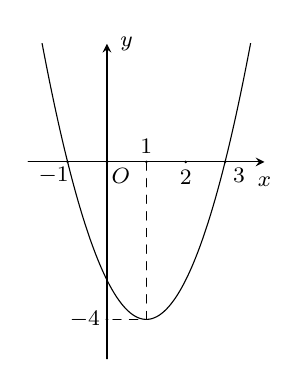
\begin{tikzpicture}[font=\footnotesize,line join=round, line cap=round, >=stealth,scale=0.5] 
\def \xmin{-2}\def \xmax{4}\def \ymin{-5}\def \ymax{3} 
\draw[->] (\xmin,0)--(\xmax,0) node[shift=(-90:0.25)] {$x$};
\draw[->] (0,\ymin)--(0,\ymax) node[shift=(0:0.25)] {$y$};
\fill (0,0) circle(1pt) node[shift=(-45:0.25)]{$O$}
(-1,0) circle(1pt) node[shift=(-135:0.25)]{$-1$}
(2,0) circle(1pt) node[shift=(-90:0.2)]{$2$}
(3,0) circle(1pt) node[shift=(-45:0.25)]{$3$}
(1,0) circle(1pt) node[shift=(90:0.2)]{$1$}
(0,-4) circle(1pt) node[shift=(180:0.28)]{$-4$};
\draw[dashed](1,0)--(1,-4)--(0,-4);
\begin{scope}
\clip (\xmin,\ymin) rectangle (\xmax,\ymax); 
\draw[smooth,samples=100,domain=\xmin:\xmax] plot(\x,{(\x)^2-2*\x-3}); 
\end{scope}
\end{tikzpicture}	
	}
\loigiai{
Dựa vào đồ thị ta có điểm $ (1,-4) \in (P)$, điểm $ (3,0) \in (P)$.\\
Suy ra $\heva{&a+b-3=-4\\&9a+3b-3=0}\Leftrightarrow \heva{&a+b=-1\\&3a+b=1}\Leftrightarrow \heva{&a=1\\&b=-2.}$\\
Vậy $ T=2a-b=2\cdot 1-(-2) =4$.
}
\end{bt}

\begin{bt}%[0T5B4-1]%[Dự án đề kiểm tra HKII NH22-23- Lương Như Quỳnh]%[Trường THPT Tenlơman]
	Cho ba điểm $ A$, $B$, $C $ thỏa mãn $ AB=3 $, $ AC=7 $, $ BC=4 $. Tính $ \overrightarrow{BC}\cdot \overrightarrow{BA} $.
\loigiai{
Ta có $ AB+BC=AC $ (vì $3+4=7$) suy ra ba điểm $ A $, $ B $, $ C $ thẳng hàng và $ B $ nằm giữa $ A $ và $ C $.
\begin{center}
\begin{tikzpicture}[font=\footnotesize,line join=round, line cap=round, >=stealth,scale=0.75] 
	\path (0,0) coordinate (A)
	(3,0) coordinate (B)
	(7,0) coordinate (C)
	;
	\draw (A)--(B)--(C)--cycle;
	\foreach \t/\g in {A/180,B/90,C/0}{
	\draw[fill=black] (\t) circle (1pt) node[shift={(\g:7pt)},font=\scriptsize]{$ \t $};
		}	
	\end{tikzpicture}
\end{center}
Do đó $ \overrightarrow{BC}\cdot \overrightarrow{BA}=BC \cdot BA \cdot \cos \left(\overrightarrow{BC},\overrightarrow{BA}\right)=4\cdot 3\cdot 180^\circ =-12$.
}
\end{bt}

\begin{bt}%[0T5B2-5]%[Dự án đề kiểm tra HKII NH22-23- Lương Như Quỳnh]%[Trường THPT Tenlơman]
	Cho hai lực $ \overrightarrow{F}_1 =\overrightarrow{MA}$, $ \overrightarrow{F}_2 =\overrightarrow{MB}$ cùng tác động vào vật tại một điểm $ M $, cường độ hai lực $ \overrightarrow{F}_1 $, $ \overrightarrow{F}_2 $ lần lượt $ 300 $ (N) và $ 400 $ (N), $ \widehat{AMB}=90^\circ $. Hãy tìm cường độ của lực tổng hợp tác động vào vật.
\loigiai{
\immini{
Gọi $ I $ là trung điểm của $ AB $.\\
Cường độ của lực tổng hợp tác động vào vật là 
\[\left| \overrightarrow{F}\right|=\left| \overrightarrow{F}_1+\overrightarrow{F}_2\right|=\left| \overrightarrow{MA}+\overrightarrow{MB}\right|=2\left| \overrightarrow{MI}\right|=AB.\]
Ta có $ AB=\sqrt{MA^2+MB^2}=500 $ suy ra $ \left| \overrightarrow{F}\right|=500 $ (N).
}
{
\tikzset{
	ex_markstyle/.style={},
	ex_mark/.style  n args={1}{decoration={ markings, %
			mark= at position 0.5 with
			with{
				\ifnum#1=1
				\draw[ex_markstyle] (0pt,-2pt) -- (0pt,2pt);
				\fi
				\ifnum#1=2
				\draw[ex_markstyle] (-1pt,-2pt) -- (-1pt,2pt);
				\draw[ex_markstyle] (1pt,-2pt) -- (1pt,2pt);
				\fi
				\ifnum#1=3
				\draw[ex_markstyle] (-2pt,-2pt) -- (-2pt,2pt);
				\draw[ex_markstyle] (0pt,-2pt) -- (0pt,2pt);
				\draw[ex_markstyle] (2pt,-2pt) -- (2pt,2pt);
				\fi
				\ifnum#1=4
				\draw[ex_markstyle] (-1pt,-1pt) -- (1pt,1pt);
				\draw[ex_markstyle] (-1pt,1pt) -- (1pt,-1pt);
				\fi
		} },
		pic actions/.append code=\tikzset{postaction=decorate}},
}
\begin{tikzpicture}[font=\footnotesize,line join=round, line cap=round, >=stealth,scale=0.75] 
	\path (0,0) coordinate (M)
	(0,4) coordinate (B)
	(3,0) coordinate (A)
	($ (B)!.5!(A) $)coordinate (I)
	;
	\draw[->] (M)--(A);
	\draw[->] (M)--(B);
	\draw[->] (M)--(I);
	\draw (A)--(B);
	\foreach \t/\g in {A/-90,B/180,M/-90,I/45}{
	\draw[fill=black] (\t) circle (1pt) node[shift={(\g:7pt)},font=\scriptsize]{$ \t $};
	\node[left]  at (0,2) {$\overrightarrow{F}_2$};
	\node[below]  at (1.5,0) {$\overrightarrow{F}_1$};
	\draw  pic[draw=black, angle eccentricity=2, angle radius=0.25cm]
	{right angle=B--M--A}; %Góc vuông
		}	
	\end{tikzpicture}
}
}
\end{bt}